\usetikzlibrary{calc}

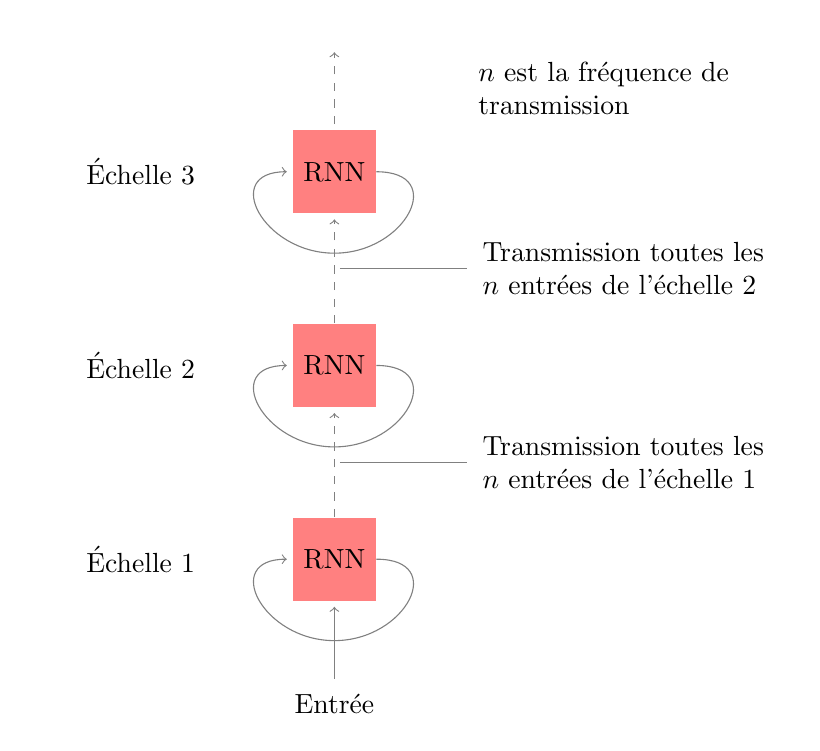
\begin{tikzpicture}[shorten >=2pt,->,draw=black!50, node distance=7em]
    \tikzstyle{every pin edge}=[<-,shorten <=2pt]
	\tikzstyle{module}=[minimum size=3em, fill=gray!50!]
	\tikzstyle{char}=[module, circle, fill=green!50!]
	\tikzstyle{text label}=[rectangle, text centered, text width=7.5em, node distance=7em]
	\tikzstyle{nn}=[rectangle, module, fill=orange!50!]
	\tikzstyle{rnn}=[nn, fill=red!50!]

	\node[rnn, pin={[pin edge={<-}, pin distance=3em]south:Entr\'{e}e}] (rnn1) {RNN};
	\node[rnn, above of=rnn1] (rnn2) {RNN};
	\node[rnn, above of=rnn2, pin={[pin edge={->,dashed}, pin distance=3em]north:}] (rnn3) {RNN};

	\foreach \n in {1,...,3}
		\draw[->] (rnn\n.east) to [out=0,in=0, looseness=2] ($(rnn\n.south) + (0,-.5)$) to [out=180,in=180, looseness=2] (rnn\n.west);

	\path[->,dashed] (rnn1)  edge coordinate (@aux) (rnn2);
	\path [late options={name=@aux, pin={[pin edge={-}, text width=10.5em, pin distance=5em]0:Transmission toutes les $n$ entr\'{e}es de l'\'{e}chelle 1}}];
	\path[->,dashed] (rnn2)  edge coordinate (@aux) (rnn3);
	\path [late options={name=@aux, pin={[pin edge={-}, text width=10.5em, pin distance=5em]0:Transmission toutes les $n$ entr\'{e}es de l'\'{e}chelle 2}}];

	\foreach \n in {1,...,3}
	    \node[text label, left of=rnn\n] (rnn\n l) {\'{E}chelle \n};
	\node[right of=rnn3, node distance=10.7em, text width=11em, yshift=3em] (rnn l) {$n$ est la fr\'{e}quence de transmission};
\end{tikzpicture}